% ---------------------------------------------------------
% Project: PhD KAPPA
% File: results.4.tex
% Author: Andrea Discacciati
%
% Purpose: Paper IV (results)
% ---------------------------------------------------------

\section{Paper IV}

Aim of this paper was to summarize the existing epidemiologic evidence --- available as aggregated data --- on the dose--response association between BMI and the incidence of localized and aggressive prostate cancer. Furthermore, possible differences in the dose--response association according to study-level covariates were investigated. Only prospective studies were included in this meta-analysis.

\subsection{Main results}

\subsubsection{Random-effect dose--response meta-analysis}

For localized prostate cancer, we observed a 6\% decreased incidence for every 5-unit increment in BMI [RR: 0.94 (95\% CI: 0.91--0.97)]. No evidence of a non-linear relationship was found when BMI was modeled using a quadratic polynomial ($p_{\textrm{non-linearity}}=0.10$). In the linear model, there was no evidence of heterogeneity ($p_{\textrm{heterogeneity}}=0.27$, $I^2=18\%$) or publication bias ($p_{\textrm{publication bias}}=0.35$ from the Egger's test).

For advanced prostate cancer, we found a 9\% increased incidence for every 5-unit increment in BMI [RR: 1.09 (95\% CI: 1.02--1.16)]. Again, no evidence of non-linearity was observed ($p_{\textrm{non-linearity}}=0.10$). There was, however, a moderate amount of between-study heterogeneity ($p_{\textrm{heterogeneity}}=0.08$, $I^2=38\%$) and evidence of publication bias ($p_{\textrm{publication bias}}=0.02$). A large part of the observed heterogeneity was due to one single study conducted in Australia, that reported a RR of 1.51 (95\% CI: 1.14--2.01) \citep{macinnis_body_2003}. Removing this study led to a decrease in the between-study variability ($p_{\textrm{heterogeneity}}=0.26$, $I^2=18\%$), while the pooled RR for every 5-unit increment in BMI changed only marginally [RR: 1.07 (95\% CI: 1.01--1.13)]. 

\subsubsection{Meta-regression and sensitivity analysis}

By means of meta-regression, we assessed whether the dose--response associations differed according to the following study-level characteristics: method of BMI collection (trained personnel versus self-reported measurements), and degree of adjustment (adjustment for physical activity and personal history of diabetes versus adjustment for only one or neither of these covariates). However, we did not observe evidence of effect modification by these study-level covariates, neither for localized nor for advanced prostate cancer.

Since the dose--response meta-analysis could have been sensitive to the choice of the BMI level assigned to the open-ended categories \citep{crippa_letter_2015}, we carried out a sensitivity analysis assuming that the amplitude of the open-ended categories was twice that of the neighborhood categories. In this scenario, the RRs for every 5-unit increment in BMI were observed to be 0.95 (95\% CI: 0.93--0.98) and 1.07 (95\% CI: 1.01--1.13) for localized and advanced prostate cancer, respectively.

Lastly, we performed a series of sensitivity analyses regarding the classification criteria used in some of the studies. First, in the meta-analysis on localized prostate cancer, we pooled the results for `moderate grade' (Gleason score 5--7) with those for `low grade' prostate cancer (Gleason score 2--4) in the study by \citet{macinnis_body_2003}. Second, in the meta-analysis on advanced prostate cancer, we pooled the results for `non-metastatic high grade' with those for `stage D or fatal' cases in the study by \citet{rodriguez_body_2007}. Third, we used the classification criterion based on Gleason score instead of the that based on the TNM staging system in the study by \citet{pischon_body_2008}. Fourth, we excluded from the meta-analysis on localized prostate cancer those three studies that used Gleason score as the only criterion to classify incident cases \citep{cerhan_association_1997, macinnis_body_2003, putnam_lifestyle_2000}. The pooled RRs did not appreciably change in any of these sensitivity analyses. 


\subsection{Updated dose--response meta-analysis}
\label{section:results4updated}

\subsubsection{Localized prostate cancer}

Figure \ref{fig:ss_loc} shows the 14 study-specific dose--response associations, where BMI was modeled using RCS with 3 knots positioned at the 10th, 50th, and 90th percentiles of the BMI distribution\footnote{Corresponding to 22.0, 26.1, and 32.5 \kgmsq.} (blue line) and in a linear fashion (red line). The regression model for the $i$-th study  was
\begin{equation*}
\E\left(y_{ij}\right) = \beta_{i1} \left[ g_1 \left(x_{ij}; \boldsymbol{\lambda}\right) - g_1 \left(x_{i0}; \boldsymbol{\lambda}\right) \right] + \beta_{i2} \left[ g_2 \left(x_{ij}; \boldsymbol{\lambda}\right) - g_2 \left(x_{i0}; \boldsymbol{\lambda}\right) \right],
\end{equation*}
for $i=1,\ldots,14$ and $j=1,\ldots,J_i$. The functions $g_1(\cdot)$ and $g_2(\cdot)$ were the 2 RCS transformations characterized by the vector $ \boldsymbol{\lambda}$ containing the knots position.

The 14 vectors of study-specific regression coefficients $\boldsymbol{\beta}_i$ were then pooled using the random-effect bivariate meta-analysis model
\begin{equation*}
\begin{pmatrix}
\beta_{i1} \\ \beta_{i2}
\end{pmatrix} \sim \N_2 \left(
\begin{pmatrix}
\theta_{1} \\ \theta_{2}
\end{pmatrix}, 
\begin{bmatrix}
\hat{\mathrm{V}}(\beta_{i11}) & \hat{\mathrm{V}}(\beta_{i12}) \\
 \hat{\mathrm{V}}(\beta_{i21}) & \hat{\mathrm{V}}(\beta_{i22})
\end{bmatrix} + 
\begin{bmatrix}
\psi_{11} & \psi_{12} \\
 \psi_{21} & \psi_{22}
\end{bmatrix} \right),
\end{equation*}
whose parameters were estimated by REML.

\begin{figure}[p]
\centering
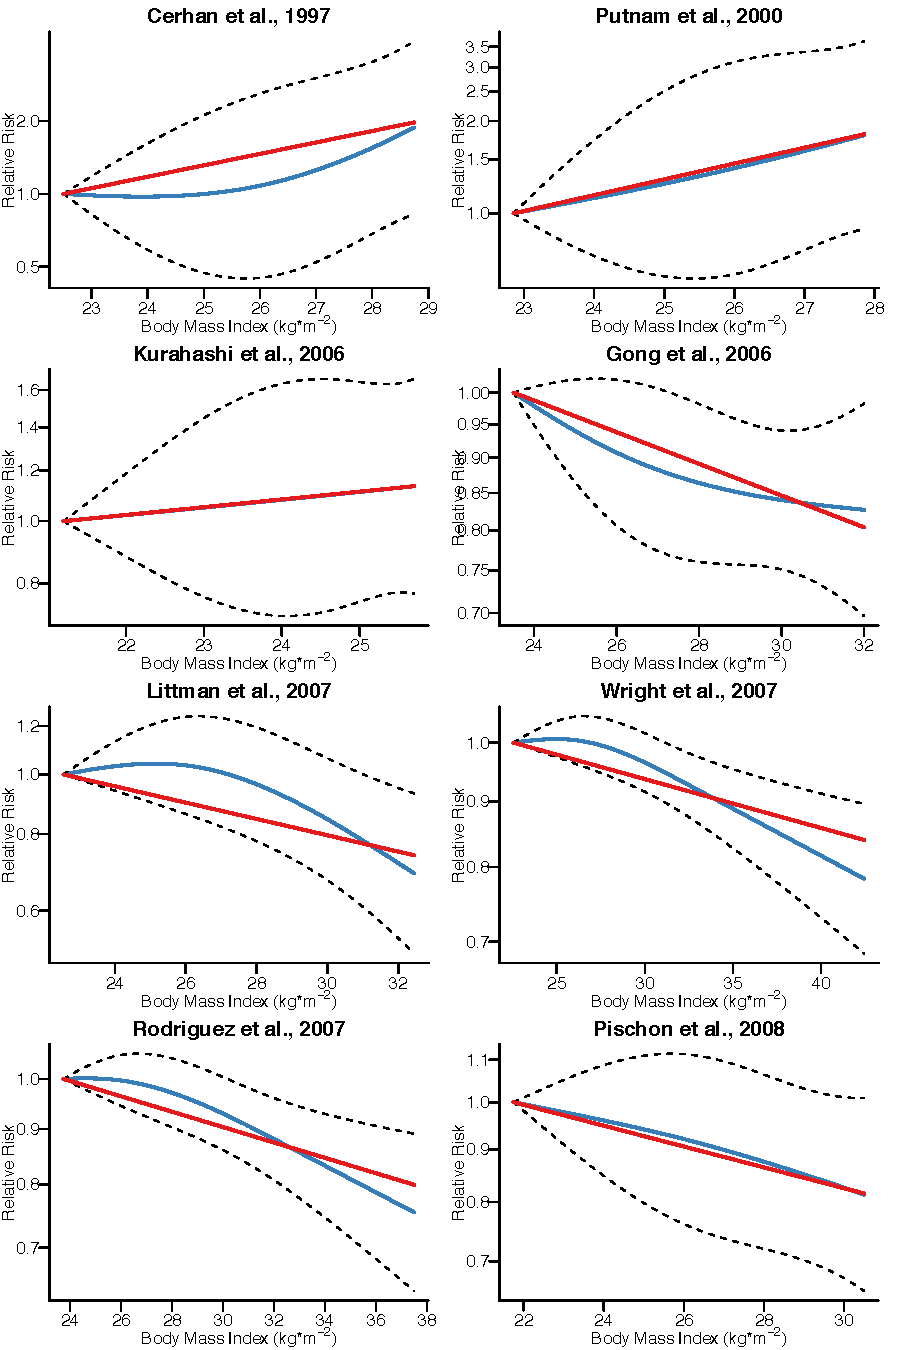
\includegraphics[width=\linewidth]{figures/ss_loc1.pdf}
\caption[Study-specific dose--response associations between BMI and incidence of localized prostate cancer]{Study-specific dose--response associations between BMI and incidence of localized prostate cancer in the updated meta-analysis including 14 prospective studies. BMI was modeled using RCS with 3 knots positioned at the 10th, 50th, and 90th percentiles of the overall BMI distribution (blue line) and in a linear fashion (red line). Dashed black lines represent the 95\% CI for the RCS models. The vertical axes are on the natural log scale. Figure continued on next page.}
\label{fig:ss_loc}
\end{figure}


\begin{figure}[p]
\centering
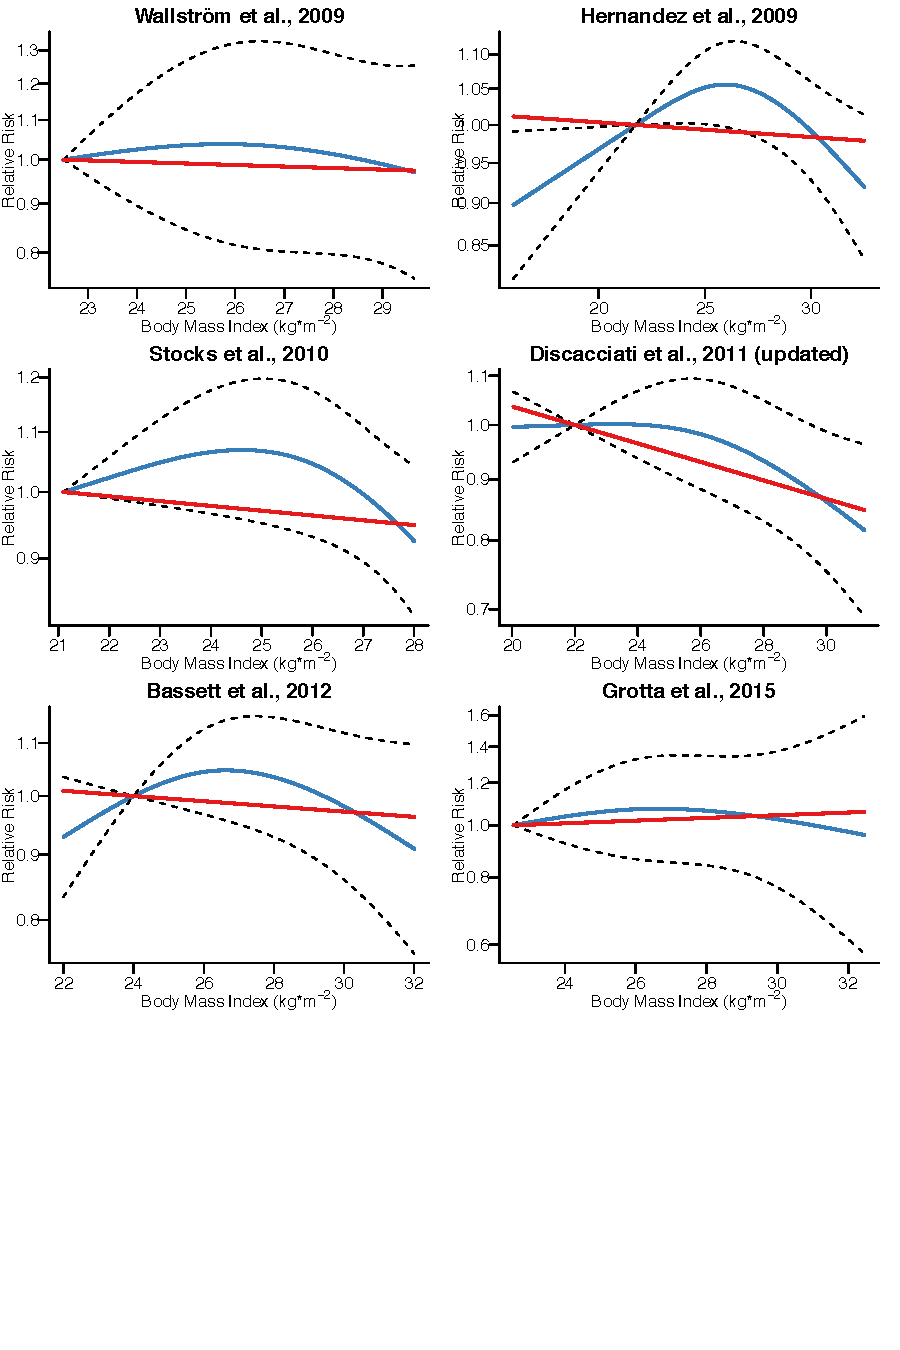
\includegraphics[width=\linewidth]{figures/ss_loc2.pdf}
\end{figure}

Overall, BMI was associated with the incidence of localized prostate cancer in the RCS model ($p_{\textrm{overall}}<0.001$) and evidence of non-linearity was observed ($p_{\textrm{non-linearity}}<0.001$), as illustrated in figure \ref{fig:pool_loc} (blue line). Compared with a BMI of 22 \kgmsq{}, the pooled RRs were 1.01 (95\% CI: 0.99--1.04) for 25 \kgmsq{}, 0.93 (95\% CI: 0.90--0.98) for 30 \kgmsq{}, and 0.81 (95\% CI: 0.74--0.88) for 35 \kgmsq{}. Between-study heterogeneity was marginal ($p_{\textrm{heterogeneity}}=0.28$, $I^2=12\%$), as measured by the multivariable extensions of the Q test and of the $I^2$ statistic [equations (\ref{eq:multiq}) and (\ref{eq:multii2})]. BMI was also modeled using RCS with knots placed at the 25th, 50th, and 75th percentiles of the BMI distribution\footnote{Corresponding to 22.8, 26.1, and 28.8 \kgmsq.} (purple line) and a quadratic polynomial (green line), as in \citetalias{discacciati_body_2012}. These 2 alternative exposure transformations gave very similar results as compared with the main analysis, both in terms of predicted population-average dose--response associations and between-study heterogeneity. Lastly, excluding the study by \citet{gong_obesity_2006}, which did not report enough data to approximate the covariance between the logRR estimates, did not virtually change the pooled dose--response association, while the between-study heterogeneity decreased to $I^2=3\%$ ($p_{\textrm{heterogeneity}}=0.42$).


\begin{figure}[h]
\centering
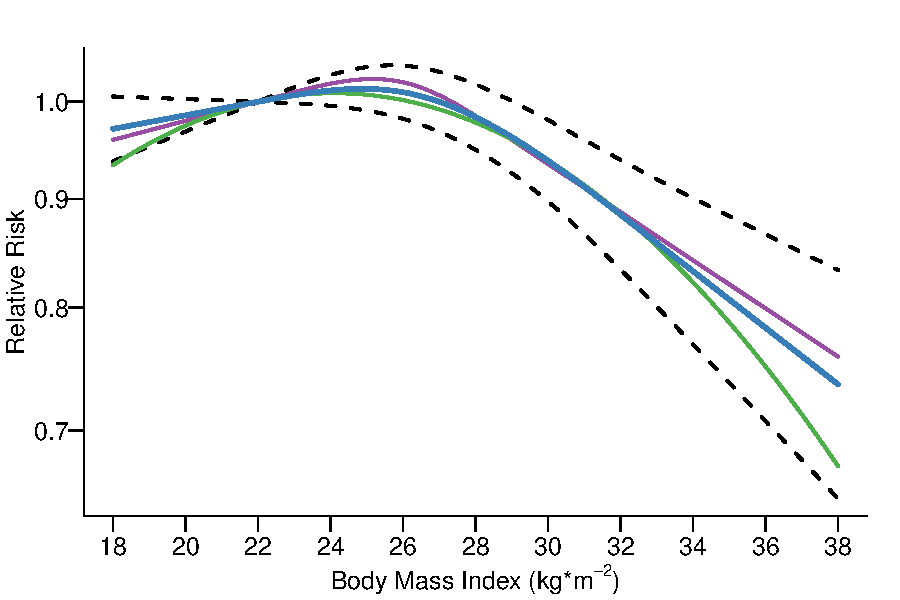
\includegraphics[width=\linewidth]{figures/pool_loc.pdf}
\caption[Pooled dose--response association between BMI and incidence of localized prostate cancer from a random-effect multivariate meta-analysis]{Pooled dose--response association between BMI and incidence of localized prostate cancer from a random-effect multivariate meta-analysis. BMI was modeled using RCS with 3 knots positioned at the 10th, 50th, and 90th percentiles of the BMI distribution (blue line), with RCS with 3 knots positioned at the 25th, 50th, and 75th percentiles of the BMI distribution (purple line), and with a quadratic polynomial transformation (green line). Dashed black lines represent the 95\% CI for the first RCS model. BMI equal to 22 \kgmsq{} served as the referent group. The vertical axis is on the natural log scale.}
\label{fig:pool_loc}
\end{figure}


\subsubsection{Advanced prostate cancer}

Similarly to what described before, figure \ref{fig:ss_adv} exhibits the 18 study-specific dose--response associations between BMI and incidence of advanced prostate cancer. BMI was modeled using RCS with 3 knots positioned at the 10th, 50th, and 90th percentiles of the BMI distribution\footnote{Corresponding to 22.0, 26.0, and 31.6 \kgmsq.} (blue line) and in a linear fashion (red line). The 18 vectors of study-specific regression coefficients used as the outcome in a random-effect bivariate meta-analysis model.

Although BMI was associated with the incidence of advanced prostate cancer in the multivariate model pooling the study-specific RCS regression coefficients ($p_{\textrm{overall}}=0.004$), no evidence of non-linearity was observed  ($p_{\textrm{non-linearity}}<0.89$) (figure \ref{fig:pool_adv}, blue line). For this reason, study-specific regression coefficients where BMI was modeled in a linear fashion were pooled by means of a univariate random-effect meta-analysis. For every 5-unit increment in BMI, the incidence of advanced prostate cancer was observed to increase by 7\% [RR: 1.07 (95\% CI: 1.03--1.12)] (red line). Between-study variability was limited as compared to total variability ($p_{\textrm{heterogeneity}}=0.15$, $I^2=26\%$). Removing those two studies that did not report information about number of cases and person-years by categories of BMI did not appreciably change the results [RR: 1.08 (95\% CI: 1.03--1.13) for every 5-unit increment, $I^2=27\%$] \citep{habel_body_2000, gong_obesity_2006}. A forest plot reporting the 18 study-specific RRs for every 5-unit increment in BMI is shown in figure \ref{fig:fp_adv}.

\begin{figure}[h]
\centering
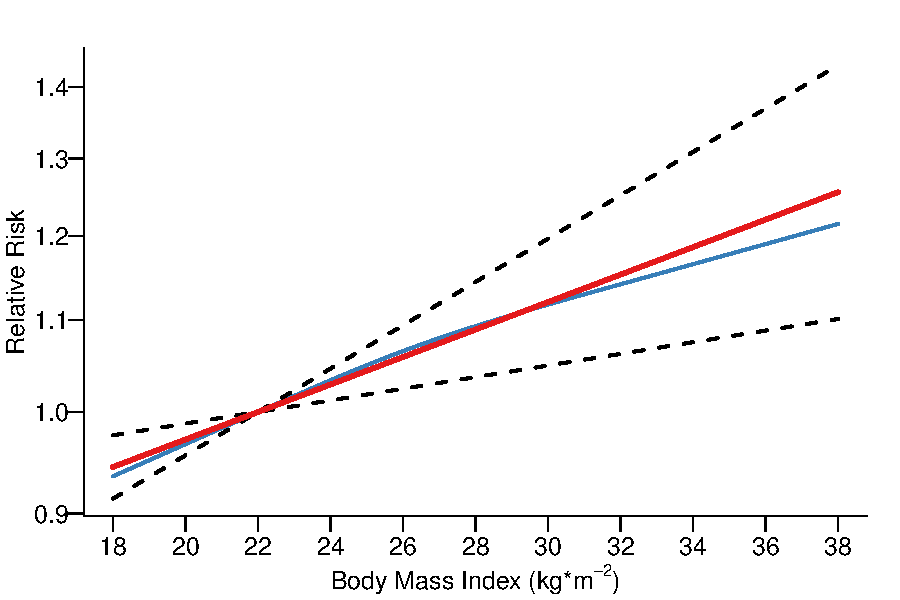
\includegraphics[width=\linewidth]{figures/pool_adv.pdf}
\caption[Pooled dose--response association between BMI and incidence of advanced prostate cancer from a random-effect multivariate meta-analysis]{Pooled dose--response association between BMI and incidence of advanced prostate cancer from a random-effect multivariate meta-analysis. BMI was modeled using RCS with 3 knots positioned at the 10th, 50th, and 90th percentiles of the BMI distribution (blue line), and in a linear fashion (red line). Dashed black lines represent the 95\% CI for the linear model. BMI equal to 22 \kgmsq{} served as the referent group. The vertical axis is on the natural log scale.}
\label{fig:pool_adv}
\end{figure}


